\chapter{Quarter-wave model simulations} \label{sec: QWSim}

As for the Valve Closing model previously, \cref{sec: Prog}, numerical simulations can be used to approximate the solution to the quarter-wave model presented in \cref{sec: QWM}.
%given in \cref{eq: FullQWMDimensionless}.
Again, the MATLAB inbuilt \textit{ode45} function is used to simulate the differential equation~\cite{Shampine1997TheSuite}, with the collisions are handled as described in \cref{sec: ValveCollision}. The numerical simulations of three different models will be considered in this section; the fixed valve quarter-wave model presented in \cref{sec: QWBehaviour}, the fixed tank pressure quarter-wave model given by \cref{eq: QWFixedTankPressure}, and finally the variable tank pressure quarter-wave model given by \cref{eq: FullQWMDimensionless}.

\section{Quarter-wave behaviour} \label{subsec: QWBehavSim}

First, %we will try to reproduce
sustained oscillations corresponding to the quarter-wave frequency using a similar analysis to in \cref{sec: QWBehaviour} will be reproduced. As before, the equations of motion are implemented such that the tank pressure remains fixed so $\dash{y_3} = 0$. Additionally, the main piston is held at the equilibrium such that $y_1 = 1$ and $\dash{y_1} = \dash{y_2} = 0$. \Cref{fig: QWMBehaviour} shows the simulation results using these conditions.
~
\begin{figure}[!ht]
    \centering
    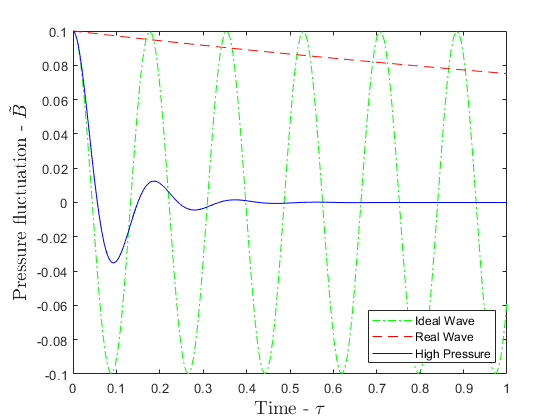
\includegraphics[width=0.7\textwidth]{Figures/QWMSimulation/QWMBehaviourB.png}
    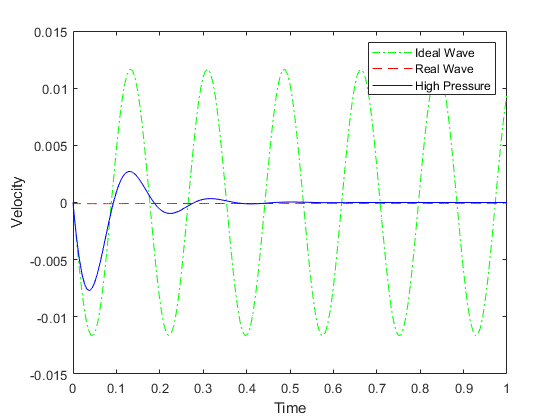
\includegraphics[width=0.7\textwidth]{Figures/QWMSimulation/QWMBehaviourC.png}
    \caption{Simulation of the quarter-wave model, \cref{eq: FullQWMDimensionless}, with a fixed tank pressure when the main piston is forced to remain in the equilibrium position ($y_1 = 1$, $y_3 = \frac{q}{\mu \sigma}$, $\dash{y_1}=\dash{y_2}=\dash{y_3}=0$). The parameters used are those in \cref{tab: ValveClosingQWMParameterValues}, except a pipe length of $L = 0.6 \, \si{m}$ is used, which corresponds to $\gamma = 0.0442$. Hence, the quarter-wave has a period of 0.1769.}
    \label{fig: QWMBehaviour}
\end{figure}

The red dashed line corresponds to the response of the pressure fluctuation for the full Quarter-Wave model. This clearly shows no signs of oscillatory motion in either the pressure or velocity fluctuations, $B(t)$ and $C(t)$ respectively. In fact, this can be explained by considering the damping which occurs when the valve is held open at $y_1 = 1$. In \cref{sec: QWBehaviour}, the linearised equation around $B(t) = C(t) = 0$ was calculated to be given by \cref{eq: QWMBehaviourTheory}. This gave a damping coefficient, expressed in dimensionless parameters and variables, of
~
\begin{equation*}
    \frac{\sqrt{2}}{4} \alpha \sigma \frac{y_1}{\sqrt{y_3}} \, .
\end{equation*}

When the values of the dimensionless parameters are used to calculate this damping coefficient, we find that the damping coefficient is $76.56$. As this is much greater than one, the second-order linear oscillator is heavily over-damped, which explains why no oscillations are seen for the quarter-wave model in \cref{fig: QWMBehaviour}.

This can be further verified when the term which contributes this damping in \cref{eq: QWMBehaviourTheory} is neglected from the simulation. Equivalently, the same behaviour can be seen by setting $\alpha \sigma = 0$. The green dotted-dashed line in \cref{fig: QWMBehaviour} shows this case, for which there is clearly oscillatory behaviour, corresponding to the quarter-wave frequency.

Let us now consider the case for which this damping term decreases because of an increasing pressure which the tank is fixed at. The solid blue line in \cref{fig: QWMBehaviour} demonstrates the extremely severe case for which the tank is held at a pressure of $y_3 = 10,000$. The damping coefficient predicts that increase the tank pressure reduces the damping which the pressure and velocity fluctuations experience. When this pressure is used, it can be calculated that the damping coefficient is $0.3144$ so the system is underdamped. \Cref{fig: QWMBehaviour} demonstrates that at a tank pressure of $y_3 = 10,000$, the system does behave as an underdamped oscillator.

The damping which acts of the quarter-wave model is also present for a direct spring-operated PRV when the valve is fixed open. However, for an equivalent direct-spring operated PRV, the corresponding $\alpha$ and $\sigma$ are significantly smaller~\cite{Hos2015DynamicModelling}. This would the quarter-wave would experience a smaller damping for a spring-operated PRV than for a pilot-operated PRV, which may help explain why chatter instability is a lesser observed event for pilot-operated PRVs.

It is also worth noting that the damping does not occur if the main piston is fixed in the closed position, such that $y_1 = 0$. This is consistent with the damping coefficient, which decreases linearly with valve position. As the damping decreases with the main piston lift, it perhaps suggests that a quarter-wave oscillation is more likely to grow unstably for small piston lifts, or when the main valve is nearly closed. This is certainly the case for direct spring-operated PRVs~\cite{Hos2017DynamicRecommendations}, so perhaps a similar effect occurs for pilot-operated PRVs.

%\newpage
%%%%%%%%%%%%%%%%%%%%%%%%%
%% FIXED TANK PRESSURE %%
%%%%%%%%%%%%%%%%%%%%%%%%%
\section{Fixed tank pressure}

Next, the main piston will be allowed to freely move based on the fluid forces that act upon it. However, the tank pressure remain fixed, which is realistic if tank is sufficiently large so the limit $V \rightarrow \infty$ implies that $\beta \rightarrow 0$. This corresponds to the fixed tank pressure model described by \cref{eq: QWFixedTankPressure}. The first simulation will be performed with the tank held at $p_0 = 0.2$ and the pipe length given by $\gamma = 2$. From the blue cross [\textcolor{Blue}{x}] in \cref{fig: BifurcationDiagram}, the dynamics are expected to be those of a stable valve closing. \Cref{fig: StableHopf} shows the time trajectories of the system.
~
\begin{figure}[ht]
    \centering
    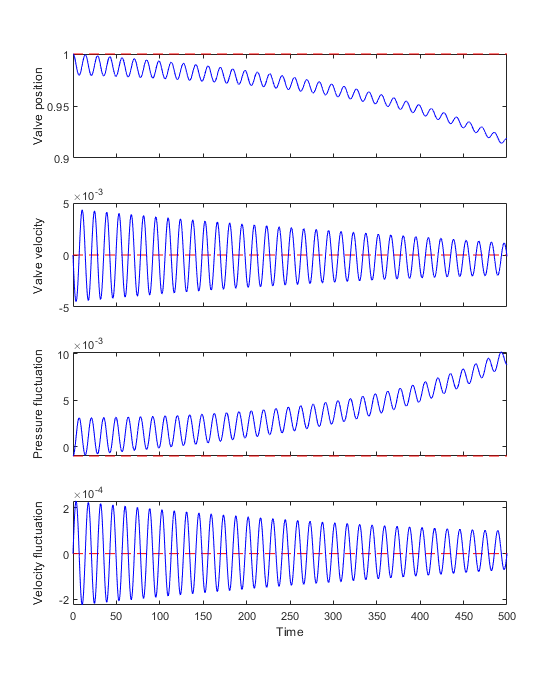
\includegraphics[width=0.7\textwidth]{Figures/CloseToHopf/HopfStable.png}
    \caption{Simulation of the fixed tank pressure quarter wave model, \cref{eq: QWFixedTankPressure}, for $\gamma = 2$ and $p_0 = 0.1$. This can be seen as a blue cross [\textcolor{Blue}{x}] in \cref{fig: BifurcationDiagram}. The other parameters are as in \cref{tab: ValveClosingQWMParameterValues}, except $\Lambda=0$ and $\phi=0$.}
    \label{fig: StableHopf}
\end{figure}

It is clear that prolonged oscillations do occur, which may be expected as, in the two-parameter space, the parameters lie near the Hopf bifurcation. However, the velocity fluctuations described by $C$ clearly show that these oscillations slowly decay. Additionally, the magnitude of the oscillations in the piston dynamics ($y_1$) also reduce in amplitude. Hence, in this region of the $\gamma$-$p_0$ parameter space, any oscillations are expected to decay and chatter will not occur.

If the simulation is continued for a longer time, it can be verified that these oscillations eventually decay such that they are no longer noticeable. Additionally, the main piston continues to diverge from the unstable equilibrium, to eventually impact with the lower stop. Hence,
%it would expected that
the valve would eventually close after a series of low energy collisions with the lower stop.

One interesting question raised by \cref{fig: StableHopf} is the frequency of the oscillations which occur. From the pipe length of $\gamma = 2$, the period of the quarter-wave oscillations is calculated to be $8$ dimensionless time units. However, the oscillations in \cref{fig: StableHopf} have a different period of approximately $10.9$ dimensionless time units. The reason for this shift in period has not yet been determined.
%
%TALK ABOUT PERIOD OF 10.9 BUT QW PERIOD OF 8?

Next, the pipe length parameter $\gamma$ is increased beyond where the Hopf bifurcation has occurred, but the tank pressure remains unchanged at $p_0 = 0.2$. This can be seen as the red diamond [\textcolor{Red}{$\diamond$}] in \cref{fig: BifurcationDiagram}, which now lies beyond the stability boundary. This increase in pipe length corresponds to an increase of the pipe length by about $27 \si{m}$ in dimensional units. \Cref{fig: UnstableHopf(Long)} shows the time trajectories of each variable for this case. 
~
\begin{figure}[ht]
    \centering
    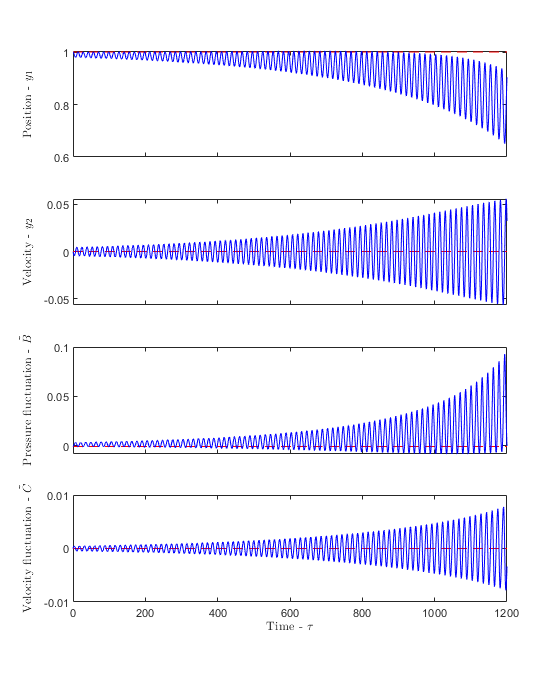
\includegraphics[width=0.7\textwidth]{Figures/CloseToHopf/HopfUnstableLong.png}
    \caption{Simulation of the fixed tank pressure quarter wave model, \cref{eq: QWFixedTankPressure}, for $\gamma = 4$ and $p_0 = 0.1$. This can be seen as a red diamond [\textcolor{Red}{$\diamond$}] in \cref{fig: BifurcationDiagram}. The other parameters are as in \cref{tab: ValveClosingQWMParameterValues}, except $\Lambda=0$ and $\phi=0$.}
    \label{fig: UnstableHopf(Long)}
\end{figure}

From the pressure and velocity fluctuations in the pipe, $B$ and $C$ respectively, it is clear that the amplitude of oscillation grows unlike for the shorter pipe length. However, the dynamics of the main piston position, $y_1$, are particularly interesting. Clearly, the amplitude of the oscillations still increases over time, but the main piston still travels downwards, diverging from from the unstable equilibrium faster than the oscillations grow. Hence, the main piston never reaches a greater height than the initial height.

\newpage
The best description of these dynamics is a flutter instability occurring. Clearly, oscillations grow in time, however not sufficiently to influence the closing of the main valve. This offers a potential explanation of why chatter instability is less apparent in pilot-operated PRVs than direct spring-operated PRVs.
For the pilot-operated PRV, the speed at which the valve closes is dependent on the unstable manifold. For a direct-spring operated case, it is dependent on how quickly the stable equilibrium approaches zero, determined by the mass flow rate.
% For the spring-operated case, the flutter oscillations are around a stationary formerly stable steady state. However, for the pilot-operated case, the flutter oscillations occur around the unstable manifold of the unstable equilibrium.
Hence, this case (\cref{fig: UnstableHopf(Long)}) of chatter not occurring is analogous to flutter not occurring for a spring-operated PRV if the flow rate changes sufficiently quickly~\cite{Hos2017DynamicRecommendations}, such that the valve closes quickly.

TALK ABOUT PERIOD OF 10.9 BUT QUARTER-WAVE PERIOD OF 16?

\Cref{fig: QWSustOsc} shows the situation which is deliberately chosen to lie on the analytically calculated stability boundary discussed in \cref{subsec: QWMAnalyticalBound}. The parameter values chosen give a value of $1 - \frac{\pi}{2} \frac{\alpha}{\gamma} = 0.1$, so the pipe is slightly over the critical pipe length required for the instability to occur. The pressure is chosen such that the other inequality for stability is exactly satisfied.
~
\begin{figure}[ht]
    \centering
    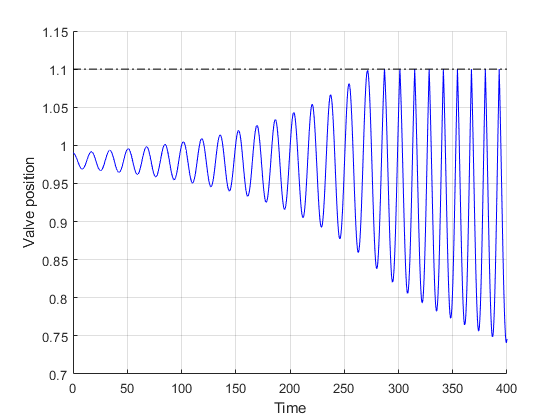
\includegraphics[width=0.49\textwidth]{Figures/QWMSimulation/SustOscilWithImpact/ValvePosition.png}
    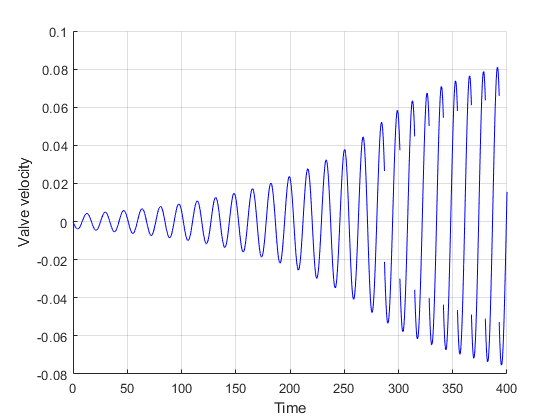
\includegraphics[width=0.49\textwidth]{Figures/QWMSimulation/SustOscilWithImpact/Velocity.png}
    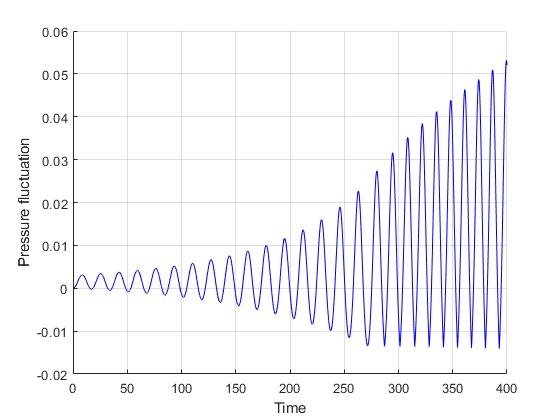
\includegraphics[width=0.49\textwidth]{Figures/QWMSimulation/SustOscilWithImpact/B.png}
    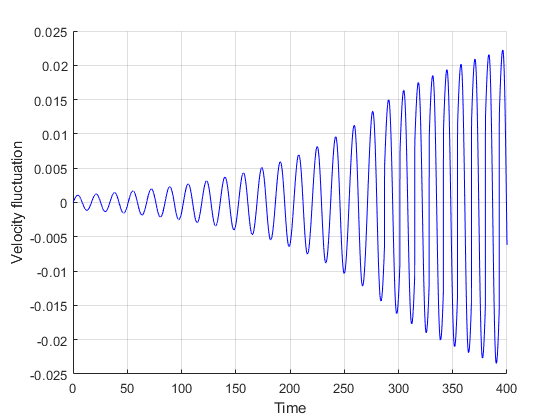
\includegraphics[width=0.49\textwidth]{Figures/QWMSimulation/SustOscilWithImpact/C.png}
    \caption{Simulation of QW with $\gamma = 14.9501$, $q = 0.6$, $\Lambda = 0$, $\alpha = 8.5658$, $\delta = 1$, $\kappa = 0$, $\beta = 0$, $\mu = 0.1407$, $\sigma = 10.3808$, $\phi = 0$ and $r = 0.8$. Equilibrium pressure is $p = 0.1686$ but the tank is actually held at $p = 0.0703$. Pressure comes from close to calculated instability boundary.}
    \label{fig: QWSustOsc}
\end{figure}

The simulation using $\gamma = 14.9501$ and $p_0 = 0.0351$ reveals one way in which the fluid dynamics within the pipe can affect the valve closing. In fact, for this given pipe length and tank pressure, the valve does not operate as desired and close as it should. Instead, the presence of a quarter-wave means some sustained oscillations occur around the unstable equilibrium lift. These oscillations most likely grow either because of the unstable eigenvalue which causes the valve to close, the non-linearity or a combination of the two effects.

Additionally, for the simulation in \cref{fig: QWSustOsc}, both the convective effects and frictional pipe losses are neglected by setting $\Lambda = 0$ and $\phi = 0$. If the convective and frictional effects are included, they dampen any sustained oscillations that occur. The valve dynamics are then dominated by the valve closing dynamics, and hence almost no oscillations can be seen.

On looking at the frequency of oscillation in \cref{fig: QWSustOsc}, these oscillations do not occur at the quarter-wave frequency. This is a confusing result as the fluid effects are only modelled using a quarter-wave frequency. It also disagrees with the limited experimental results which have been performed on a pilot-operated PRV~\cite{Allison2015TestingValves}.

%%%%%%%%%%%%%%%%
%% FULL MODEL %%
%%%%%%%%%%%%%%%%
\section{Variable tank pressure}

Finally, the case for which the full quarter-wave model, \cref{eq: FullQWMDimensionless}, will be considered. As before for \cref{fig: QWSustOsc}, the convective effects and frictional pipe losses will be ignored by setting $\Lambda = 0$ and $\phi = 0$. The parameters chosen correspond to a pipe length of $L = 20 \si{m}$, with a mass inflow to the tank of $2.28 \, \si{kg.s^{-1}}$. \Cref{fig: QWNearEquil} shows these results.
%for the full quarter-wave model described by \cref{eq: FullQWMDimensionless}.
~
\begin{figure}[!ht]
    \centering
    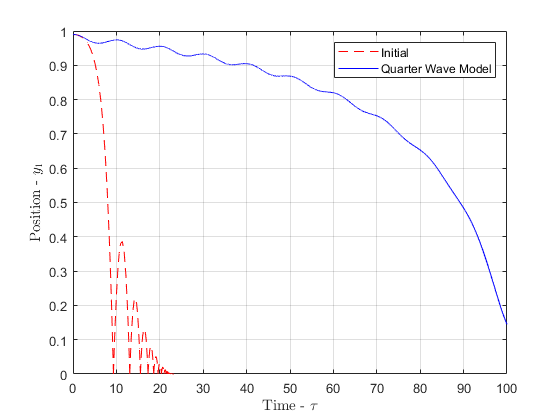
\includegraphics[width=0.4\textwidth]{Figures/QWMSimulation/NearEquilibriumOscillations/Position.png}
    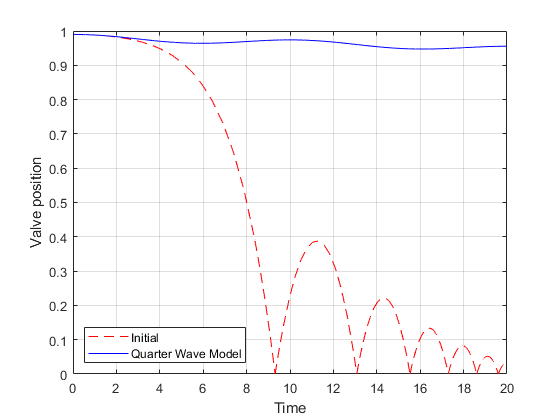
\includegraphics[width=0.4\textwidth]{Figures/QWMSimulation/NearEquilibriumOscillations/Position-Short.png}
    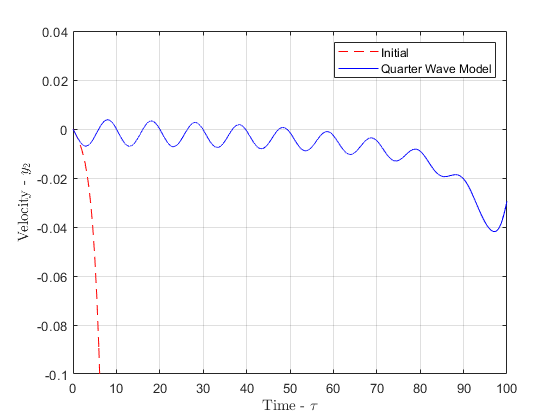
\includegraphics[width=0.4\textwidth]{Figures/QWMSimulation/NearEquilibriumOscillations/Velocity.png}
    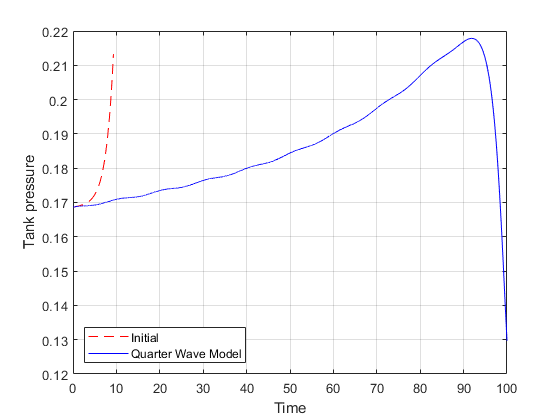
\includegraphics[width=0.4\textwidth]{Figures/QWMSimulation/NearEquilibriumOscillations/Pressure.png}
    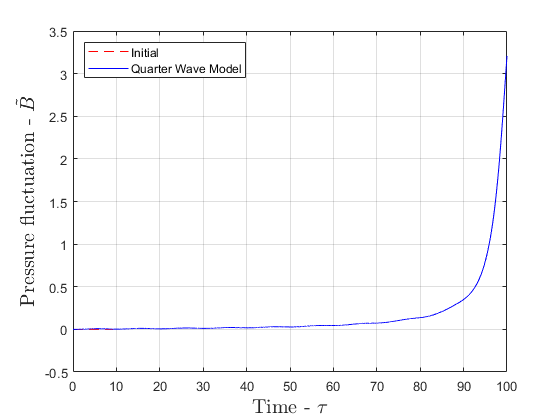
\includegraphics[width=0.4\textwidth]{Figures/QWMSimulation/NearEquilibriumOscillations/B.png}
    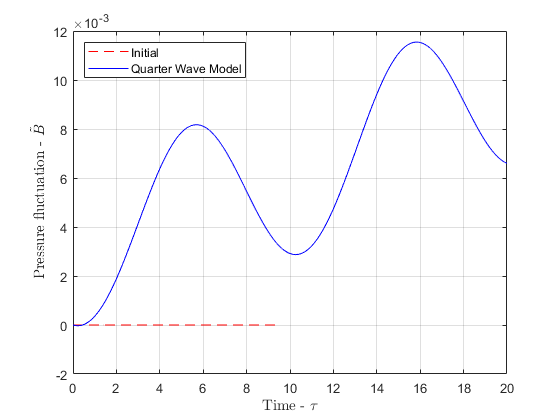
\includegraphics[width=0.4\textwidth]{Figures/QWMSimulation/NearEquilibriumOscillations/B-Short.png}
    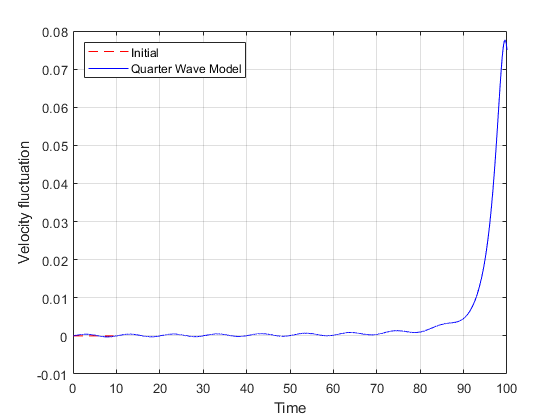
\includegraphics[width=0.4\textwidth]{Figures/QWMSimulation/NearEquilibriumOscillations/C.png}
    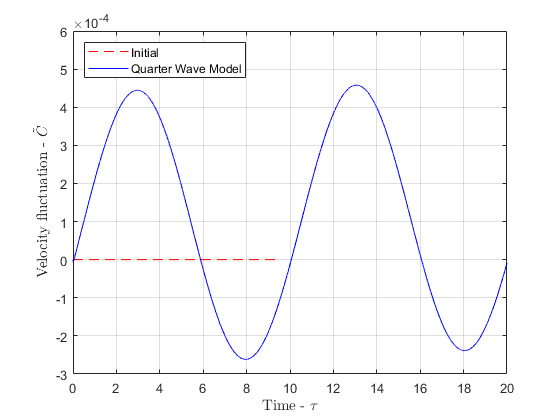
\includegraphics[width=0.4\textwidth]{Figures/QWMSimulation/NearEquilibriumOscillations/C-Short.png}
    % \caption{Simulation of QW with $\gamma = 1.4745$, $q = 0.6$, $\Lambda = 0$, $\alpha = 8.5658$, $\delta = 1$, $\kappa = 0$, $\beta = 0.0433$, $\mu = 0.1407$, $\sigma = 10.3808$, $\phi = 0$ and $r = 0.8$. The initial pressure is the equilibrium pressure of $p = 0.1686$.}
    \caption{Simulation of the full quarter wave model, \cref{eq: FullQWMDimensionless}, for $\gamma = 1.4745$. This can be seen as a blue asterisk [\textcolor{Blue}{$*$}] in \cref{fig: BifurcationDiagram}. The other parameters are as in \cref{tab: ValveClosingQWMParameterValues}, except $\Lambda=0$ and $\phi=0$. The initial conditions are equilibrium values, except $y_1(0) = 0.99$.}
    \label{fig: QWNearEquil}
\end{figure}

The first interesting point to note is for the same initial conditions, the Valve Closing model from \cref{sec: Prog} means the main piston closes within $10$ \textcolor{Red}{write in dimensional units}. However, the Quarter-Wave model closes an order of magnitude slower, taking over $100$ \textcolor{Red}{write in dimensional units} for the main valve to close.
%This is to be expected, as if the unstable behaviour of the main piston corresponding to the valve closing is too great, the dynamics will be dominated by this an oscillations do not have the opportunity to grow.

For the parameters chosen, it is clear that for a short time scale the tank pressure does remain constant. However, as the valve moves further from the unstable equilibrium, the rate of the pressure change increases. Once the main piston is almost closed, there becomes a large pressure change. This suggests that the constant pressure approximation applied in \cref{subsec: QWMAnalyticalBound} seems valid on a short time-scale. It also suggests that pressure fluctuations within the tank help to stabilise the system, as they ensure the valve still closes rather than supports sustained oscillations like in \cref{fig: QWSustOsc}. Again, we note that the oscillation frequency of the system again does not match that of the quarter-wave frequency.

The final important conclusion to be drawn from \cref{fig: QWNearEquil} is the behaviour of the pressure and velocity fluctuations, $B(t)$ and $C(t)$ respectively. In deriving the quarter-wave model, these were assumed to be small amplitude oscillations around the equilibrium. But the pressure fluctuation $B(t)$ in particular does not remain small for all time, but instead grows to an order of magnitude larger than the tank pressure as $y_1 \rightarrow 0$. Because of this, it appears the quarter-wave model will be valid close to the equilibrium, but seems less valid as the valve closes. As the main piston velocity increases in magnitude, this increases the magnitude of $\dot{v}_L(t)$. The large value of $\dot{v}_L(t)$ will likely dominate the equations for $\dash{\tilde{B} \,}$ and $\dash{\tilde{C} \,}$. One reason for this may be because the main piston's downward motion excites the quarter-wave, and if this is the case then other wave frequencies must be considered.